%
% main.tex -- Paper zum Thema <clifford>
%
% (c) 2020 Hochschule Rapperswil
%
\chapter{Thema\label{chapter:clifford}}
\lhead{Thema}
\begin{refsection}
\chapterauthor{Hans Muster}

Ein paar Hinweise für die korrekte Formatierung des Textes
\begin{itemize}
\item
Absätze werden gebildet, indem man eine Leerzeile einfügt.
Die Verwendung von \verb+\\+ ist nur in Tabellen und Arrays gestattet.
\item
Die explizite Platzierung von Bildern ist nicht erlaubt, entsprechende
Optionen werden gelöscht. 
Verwenden Sie Labels und Verweise, um auf Bilder hinzuweisen.
\item
Beginnen Sie jeden Satz auf einer neuen Zeile. 
Damit ermöglichen Sie dem Versionsverwaltungssysteme, Änderungen
in verschiedenen Sätzen von verschiedenen Autoren ohne Konflikt 
anzuwenden.
\item 
Bilden Sie auch für Formeln kurze Zeilen, einerseits der besseren
Übersicht wegen, aber auch um GIT die Arbeit zu erleichtern.
\end{itemize}

%
% einleitung.tex -- Beispiel-File für die Einleitung
%
% (c) 2020 Prof Dr Andreas Müller, Hochschule Rapperswil
%
\section{Teil 0\label{clifford:section:teil0}}
\rhead{Teil 0}
Lorem ipsum dolor sit amet, consetetur sadipscing elitr, sed diam
nonumy eirmod tempor invidunt ut labore et dolore magna aliquyam
erat, sed diam voluptua \cite{clifford:bibtex}.
At vero eos et accusam et justo duo dolores et ea rebum.
Stet clita kasd gubergren, no sea takimata sanctus est Lorem ipsum
dolor sit amet.

Lorem ipsum dolor sit amet, consetetur sadipscing elitr, sed diam
nonumy eirmod tempor invidunt ut labore et dolore magna aliquyam
erat, sed diam voluptua.
At vero eos et accusam et justo duo dolores et ea rebum.  Stet clita
kasd gubergren, no sea takimata sanctus est Lorem ipsum dolor sit
amet.



%
% teil1.tex -- Beispiel-File für das Paper
%
% (c) 2020 Prof Dr Andreas Müller, Hochschule Rapperswil
%
%
% teil2.tex -- Beispiel-File für teil2 
%
% (c) 2020 Prof Dr Andreas Müller, Hochschule Rapperswil
%%



\rhead{Kalman-Filter}

\section{Kalman-Filter}
Da wir die äussere Kraft nicht direkt messen können, benötigen wir ein Werkzeug, welches aus der gemessenen Position, die Krafteinwirkung auf unsere System schätzt. 
Dies ist eine Typische Anwendung für den linearen Kalman-Filter.
Unser Ziel ist es, anhand der Messung die eigentlich interessante Grösse $f$ zu bestimmen. 
Dabei wird durch eine deterministische Vorhersage, in dem der Zustand * Eigendynamik des Systems gerechnet. 
Die Idee dahinter ist, dass das Kalman-Filter die nicht-deterministische Grösse $f$ anhand der Messung und der Vorhersage zu bestimmen.

Für mehrere Dimensionen (x,y,z) würde der Pythagoras für das System benötigt werden.
Da sich der Pythagoras bekanntlich nicht linear verhält, kann kein lineares Kalman-Filter implementiert werden. 
Da das Kalman-Filter besonders effektiv und einfach für lineare Abläufe geeignet ist, würde eine zweidimensionale Betrachtung den Rahmen dieser Arbeit sprengen. 
Für ein nicht-lineares System werden Extended Kalman-Filter benötigt, bei denen die System-Matrix (A) durch die Jacobi-Matrix des System ersetzt wird.
Einfachheitshalber beschränken wir uns auf den linearen Fall, da dadurch die wesentlichen Punkte bereits aufgezeigt werden. 

\subsection{Geschichte}
Das Kalman-Filter wurde 1960 von Rudolf Emil Kalman entdeckt und direkt von der NASA für die Appollo Mission benutzt. Der Filter kommt mit wenig Rechenleistung aus und war somit dafür geeignet die Rakete bei der Navigation zu unterstützen. Das Filter schätzt den Zustand eines Systems anhand von Messungen und kann den nächsten Zustand errechnen. Eine typische Anwendungen des Kalman-Filters ist Glättung von verrauschten Daten und die Schätzung von Parametern. Dies kommt heutzutage in jedem Satellit, Navigationssystem, Smartphones und Videospielen vor.

\subsection{Wahrscheinlichkeit}
Das Kalman-Filter schätzt den wahrscheinlichsten Wert zwischen Normalverteilungen.
Dies bedeutet, das Filter schätzt nicht nur den Mittelwert, sondern auch die Standartabweichung.
Da Normalverteilungen dadurch vollständig definiert sind, schätzt ein Kalman-Filter die gesamte Verteilungsfunktion des Zustandes.
Die eine Funktion zeigt die errechnete Vorhersage des Zustands, bzw. deren Normalverteilung. 
Die andere Funktion zeigt die verrauschte Messung des nächsten Zustand, bzw. deren Normalverteilung. 
Wie man am Beispiel der Gauss-Verteilungen unten sehen kann, ist sowohl der geschätzte Zustand als auch der gemessene Zustand normalverteilt und haben dementsprechend unterschiedliche Standardabweichungen $\sigma$ und Erwartungswerte $\mu$.

\begin{figure}
 \begin{center}
 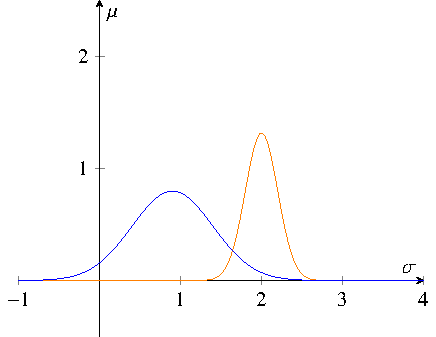
\includegraphics[width=5cm]{papers/erdbeben/Gausskurve2.pdf}
 \caption{Zwei Normalerteilungen; Die eine Funktion zeigt die Vorhersage, die andere die Messung}
 \end{center}
\end{figure}


Um eine genauere Schätzung des Zustandes zu machen, wird nun ein Wert zwischen den beiden Verteilungen berechnet. 
Nun wird eine Eigenschaft der Normalverteilung ausgenutzt. Durch das Multiplizieren zweier Normalverteilungen entsteht eine neue Normalverteilung. 
Wir haben eine Normalverteilung der Vorhersage:

\[ {y_1}(x;{\mu_1},{\sigma_1})=\frac{1}{\sqrt{2\pi\sigma_1^2}}\quad e^{-\frac{(x-{\mu_1})^2}{2{\sigma_1}^2}} \]
und der Messung:
\[ {y_2}(x;{\mu_2},{\sigma_2})=\frac{1}{\sqrt{2\pi\sigma_2^2}}\quad e^{-\frac{(x-{\mu_2})^2}{2{\sigma_2}^2}}. \]



Diesen werden nun Multipliziert und durch deren Fläche geteilt um sie wieder zu Normieren:
\[
{y_f}(x;{\mu_f},{\sigma_f})=\frac{ \frac{1}{\sqrt{2\pi\sigma_1^2}}e^{-\frac{(x-{\mu_1})^2}{2{\sigma_1}^2}} \cdot \frac{1}{\sqrt{2\pi\sigma_2^2}}e^{-\frac{(x-{\mu_2})^2}{2{\sigma_2}^2}}}{\int {y_1}\cdot{y_2} dx\,}
 \] 

Diese Kombination der beiden Verteilungen resultiert wiederum in einer Normalverteilung
\[ {y_f}(x; {\mu_f}, {\sigma_f}) = {y_1}(x;{ \mu_1},{ \sigma_1}) {\cdot y_2}(x; {\mu_2}, {\sigma_2}), \]
mit Erwartungswert
\[ \mu_f = \frac{\mu_1\sigma_2^2 + \mu_2 \sigma_1^2}{\sigma_1^2 + \sigma_2^2} \]
und Varianz
\[ \sigma_f^2 = \frac{\sigma_1^2 \sigma_2^2}{\sigma_1^2 + \sigma_2^2}. \]

Dadurch gleicht sich die neue Kurve den anderen an. Interessant daran ist, dass die fusionierte Kurve sich der genauere Normal-Verteilung anpasst.
Ist ${\sigma_2}$ klein und ${\sigma_1}$ gross, so wird sich die fusionierte Kurve näher an ${y_2}(x;{\mu_2},{\sigma_2})$ begeben.
Sie ist also gewichtet und die best mögliche Schätzung. 


\begin{figure}
 \begin{center}
 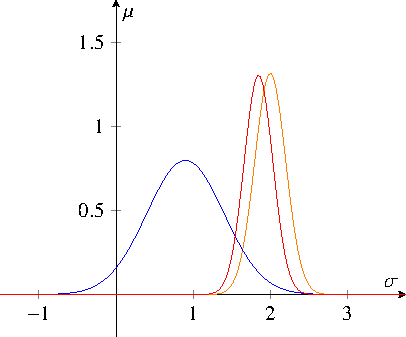
\includegraphics[width=5cm]{papers/erdbeben/Gausskurve3.pdf}
 \caption{Durch das Multiplizieren der blauen und der orangen Verteilung entsteht die die rote, optimale Funktion}
 \end{center}
\end{figure}


Was in 2 Dimensionen erklärt wurde, funktioniert auch in mehreren Dimensionen. 
Dieses Prinzip mach sich das Kalman Filter zu nutze, und wird von uns für die Erdbeben Berechnung genutzt. 

\section{Filter-Matrizen}
Um den Kalman Filter zu starten, müssen gewisse Bedingungen definiert werden. 
In diesem Abschnitt werden die einzelnen Parameter und Matrizen erklärt und erläutert, wofür sie nützlich sind. 

\subsection{Anfangsbedingungen}
\subsubsection*{Anfangszustand $x$}
Das Filter benötigt eine Anfangsbedingung. 
In unserem Fall ist es die Ruhelage, die Masse bewegt sich nicht. 
Zudem erfährt die Apparatur keine äussere Kraft.


\[ {x_0 }= \left( \begin{array}{c} {s_0}\\ {v_0}\\{f_0}\end{array}\right) = \left( \begin{array}{c} 0\\ 0\\ 0\end{array}\right) \]

\subsubsection*{Anfangsfehler / Kovarianzmatrix $P$}
Da auch der Anfangszustand fehlerhaft sein kann, wird für das Filter ein Anfangsfehler verwendet. 
Auf der Diagonalen werden die Varianzen eingesetzt, in den restlichen Felder stehen die Kovarianzen.
Zur Erinnerung: Die Varianz ist ein Mass für die Streuung eines Wertes, die Kovarianz hingegen beschreibt die Abhängigkeit der Streuungen zweier Werte.

Kovarianz: Cov(x, y) und Varianz: Var(x) = Cov(x, x)

In unserem Fall ist der Anfangszustand gut bekannt. 
Wir gehen davon aus, dass das System in Ruhe und in Abwesenheit eines Erdbeben startet, somit kann die Matrix mit Nullen bestückt werden. 
Als Initialwert für die für die Kovarianzmatrix ergibt sich

\[ 
{P_0 }=
\left(
\begin{array}{ccc} 	
0 & 0 &0 \\ 
0 &0 & 0 \\ 
0 & 0 &0 \\
\end{array}
\right).
 \] 
Diese Matrix beschreibt die Unsicherheit des geschätzten Zustandes und wird sowohl für die Vorhersage als auch die Korrektur benötigt. 
Sie wird nach jeder Schätzung aktualisiert. 
Für einen gut bekannten Zustandsvektor können kleine Werte eingesetzt werden, für ungenaue Anfangsbedingungen sollten grosse Werte verwendet werden. 
Grosse Werte ermöglichen dem Filter sich schnell einzupendeln. 

\subsubsection*{Dynamikmatrix $A$}
Das Kalman-Filter benötigt für die Vorhersage des nächsten Zustandes eine Beschreibung der Systemdynamik.
Die Dynamikmatrix bildet den Kern des Filters. Diese wurde weiter oben bereits beschrieben. 
Dabei wollen wird die äussere Kraft des Systems ermitteln.
Da nichts über die äussere Kraft bekannt ist, müssen wir annehmen das deren Ableitung 0 ist. 
Die System Vektor-Gleichung lautet daher:
\[ 
A = \left(
 \begin{array}{ccc} 	
0 & 1& 0 \\
- \frac{D}{m} &-\frac{2k}{m} & \frac{1} {m}\\
0 & 0& 0\\ 
\end{array}\right)  
 \]
Dabei soll der Kalman-Filter in diskreten Zeitschritten $\Delta t$ arbeiten. 
Die Übergangs-Matrix erhalten wir aus der Systemdynamikmatrix mittels Exponentialfunktion: 
\[\Phi = \exp(A\Delta t). \]

\subsubsection*{Prozessrauschkovarianzmatrix $Q$}
Die Prozessrauschmatrix teilt dem Filter mit, wie sich der Prozess verändert. 
Kalman-Filter berücksichtigen Unsicherheiten wie Messfehler und -rauschen. 
Bei unserem Modell könnte das beispielsweise ein Windstoss an die Masse sein. 
Für uns wäre dies:
\[ 
Q = \left(
 \begin{array}{ccc} 	
{\sigma_s }^2& 0& 0 \\ 
0 & {\sigma_v }^2& 0\\ 
0 & 0& {\sigma_f }^2\\
\end{array}\right)  
 \]

Die Standabweichungen müssten statistisch ermittelt werden, da der Fehler nicht vom Sensor kommt und somit nicht vom Hersteller gegeben ist. 
Das Bedeutet wiederum dass $Q$ die Unsicherheit des Prozesses beschreibt und nicht die der Messung.

\subsubsection*{Messmatrix $H$}
Die Messmatrix gibt an, welche Parameter gemessen werden
In unserem Falle ist es die Position der Massen. 

\[ H = (1, 0, 0) \]

\subsubsection*{Messrauschkovarianz $R$}
Die Messrauschkovarianzmatrix beinhaltet, wie der Name es schon sagt, das Rauschen der Positionsmessung. 
In unserem Fall wird nur die Position der Masse gemessen. Da wir keine anderen Sensoren haben ist $R$ lediglich:
\[ R= ({\sigma_{sensor}}^2).
 \] 
Diese Messrauchen wird meistens vom Sensorhersteller angegeben. 
Für unsere Theoretische Apparatur wird hier ein kleiner Fehler eingesetzt da heutige Sensoren sehr genau messen können. 

\subsection{Fiter-Agorithmus}
Nachdem alle Parameter aufgestellt sind, wird das Filter initialisiert.
Zuerst wird der nächste Zustand der Feder vorhergesagt, danach wird die Messung präzisiert und laufend zu aktualisieren. 
Das Filter berechnet aufgrund der aktuellen Schätzung eine Vorhersage. 
Diese wird, sobald verfügbar, mit der Messung verglichen. 
Aus dieser Differenz und den Unsicherheiten des Prozesses ($Q$) und der Messung ($R$) wird der wahrscheinlichste, neue Zustand geschätzt.

\subsubsection*{Vorhersage}
Im Filterschritt Vorhersage wird der nächste Zustand anhand des Anfangszustand und der Systemmatrix berechnet. 
Dies funktioniert mit dem Rechenschritt:
\[ 
{x_{k|k-1}}=\Phi \cdot {x_{k-1|k-1}}= \exp(A\Delta t)\cdot{x_{k|k-1}}.
 \] 

Die Kovarianz $P_{pred}$ wird ebenfalls neu berechnet. Da wir ein mehrdimensionales System haben, kommt noch die Prozessunsicherheit $Q$ dazu, so dass die Unsicherheit des Anfangsfehlers $P$ laufend verändert. 
Dies funktioniert durch multiplizieren der Systemmatrix mit dem aktualisierten Anfangsfehler. 
Dazu wird noch die Prozessunsicherheit addiert, somit entsteht die Gleichung
\[ {P_{k|k-1}} = {\Phi_k}  {P_{k-1|k-1}} {\Phi_k} ^T + {Q_{k-1}} .\] 
Es vergeht genau $dt$ Zeit, und dieser Vorgang wird wiederholt. 
Dabei wird in den späteren Schritten überprüft, wie genau die letzte Anpassung von $P$ zur Messung stimmt. 
Ist der Unterschied klein, wird die Kovarianz $P$ kleiner, ist der Unterschied gross, wird auch die Kovarianz grösser. 
Das Filter passt sich selber an und korrigiert sich bei grosser Abweichung.

\subsubsection*{Messen}
Der Sensor wurde noch nicht benutz, doch genau der liefert Werte für das Filter. 
Die aktuellen Messwerte $z$ werden die Innovation $w$ mit dem Zustandsvektor $x$ und der Messmatrix $H$ zusammengerechnet.
Hier bei wird lediglich die Messung mit dem Fehler behaftet, und die Messmatrix $H$ mit der Vorhersage multipliziert

\[{w_{k}}={z_{k}}-{H_{k}}\cdot{x_{k|k-1}}.\] 

Die Innovation ist der Teil der Messung, die nicht durch die Systemdynamik erklärt werden kann. 
Die Hilfsgröße Innovation beschreibt, wie genau die Vorhersage den aktuellen Messwert mittels der Systemmatrix $\phi$ beschreiben kann. 
Für eine schlechte Vorhersage wird die dazugehörige Innovation gross, für eine genaue Vorhersage dagegen klein sein. 
Entsprechende Korrekturen müssen dann gross bzw. nur gering ausfallen. 
Innovation = Messung - Vorhersage. Dies ist intuitiv logisch, eine Innovation von 0 bedeutet, dass die Messung nichts Neues hervorbrachte.

Im nächsten Schritt wir analysiert, mit welcher Kovarianz weiter gerechnet wird. 
Hierbei wird die Unsicherheit $P$, die Messmatrix $H$ und die Messunsicherheit $R$ miteinander verrechnet. 
\[ 
{S_{k}}={H_{k}}{P_{k|k-1}}{H_{k}}^T+{R_{k}}
 \] 

\subsubsection*{Aktualisieren}
Im nächsten Schritt kommt nun die Wahrscheinlichkeit nach Gauss dazu. 
\[ 
{K_{k}}= {{P_{k|k-1}} \cdot {H_{k}^T}}\cdot {S_{k}}^{-1} 
 \] 
Dieser Vorgang wird Kalman-Gain genannt. 
Er sagt aus, welcher Kurve mehr Vertraut werden soll, dem Messwert oder der Systemdynamik.
Das Kalman-Gain wird geringer wen der Messwert dem vorhergesagten Systemzustand entspricht. 
Sind die Messwerte komplett anders als die Vorhersage, wo werden die Elemente in der Matrix $K$ grösser.
Anhand der Informationen aus dem Kalman-Gain $K$ wird das System geupdated.

\[ 
{x_{k|k}}={x_{k|k-1}}+({K_{k}}\cdot {w_{k}}) 
 \] 

Dazu kommt  eine neue Kovarianz für den nächste Vorhersageschritt:

\[ 
{P_{k|k}}=(I-({K_{k}} \cdot {H_{k}})) \cdot {P_{k|k-1}}  
 \] 

Der ganze Ablauf wird nun zum Algorithmus und beginnt wieder mit der Vorhersage 

\[ 
{x_{k|k-1}}=\Phi \cdot {x_{k-1|k-1}}= \exp(A\Delta t)\cdot{x_{k|k-1}}.
 \] 


\subsection{Zusammenfassung }
Zusammenfassend kann das Kalman-Filter in offizieller Typus dargestellt werden. 
Dabei beginnt das Filter mit dem Anfangszustand für $k=0$

1. Nächster Zustand vorhersagen
\[{x_{k|k-1}}=\Phi \cdot {x_{k-1|k-1}}= \exp(A\Delta t)\cdot{x_{k|k-1}}.\] 

2. Nächste Fehlerkovarianz vorhersagen
\[{P_{k|k-1}}={\Phi _{k}} {P_{k-1|k-1}} {\Phi _{k}}^T + {Q_{k-1}}.\] 

3. Das Kalman Filter anwenden
\[{K_{k}}= {P_{k|k-1}} \cdot {H_{k}^T}\cdot {S_{k}^{-1}}\] 

4. Schätzung aktualisieren
\[{x_{k|k}}={x_{k|k-1}}+({K_{k}}\cdot {w_{k}}) \] 

5. Fehlerkovarianz aktualisieren
\[{P_{k|k}}=(I-({K_{k}}\cdot {H_{k}})) \cdot {P_{k|k-1}} \] 


6. Die Outputs von $k$ werden die Inputs für ${k-1}$ und werden wieder im Schritt 1 verwendet


%
% teil2.tex -- Beispiel-File für teil2 
%
% (c) 2020 Prof Dr Andreas Müller, Hochschule Rapperswil
%
\section{Fraktale mit IFS 
\label{ifs:section:teil2}}
\rhead{Teil 2}
Wollen wir nun eine bestimmte Art anschauen, wie man Fraktale machen kann.
Zur Veranschaulichung dieser Methode nehmen wir das Sierpinski Dreieck.
\begin{figure}
	\centering
	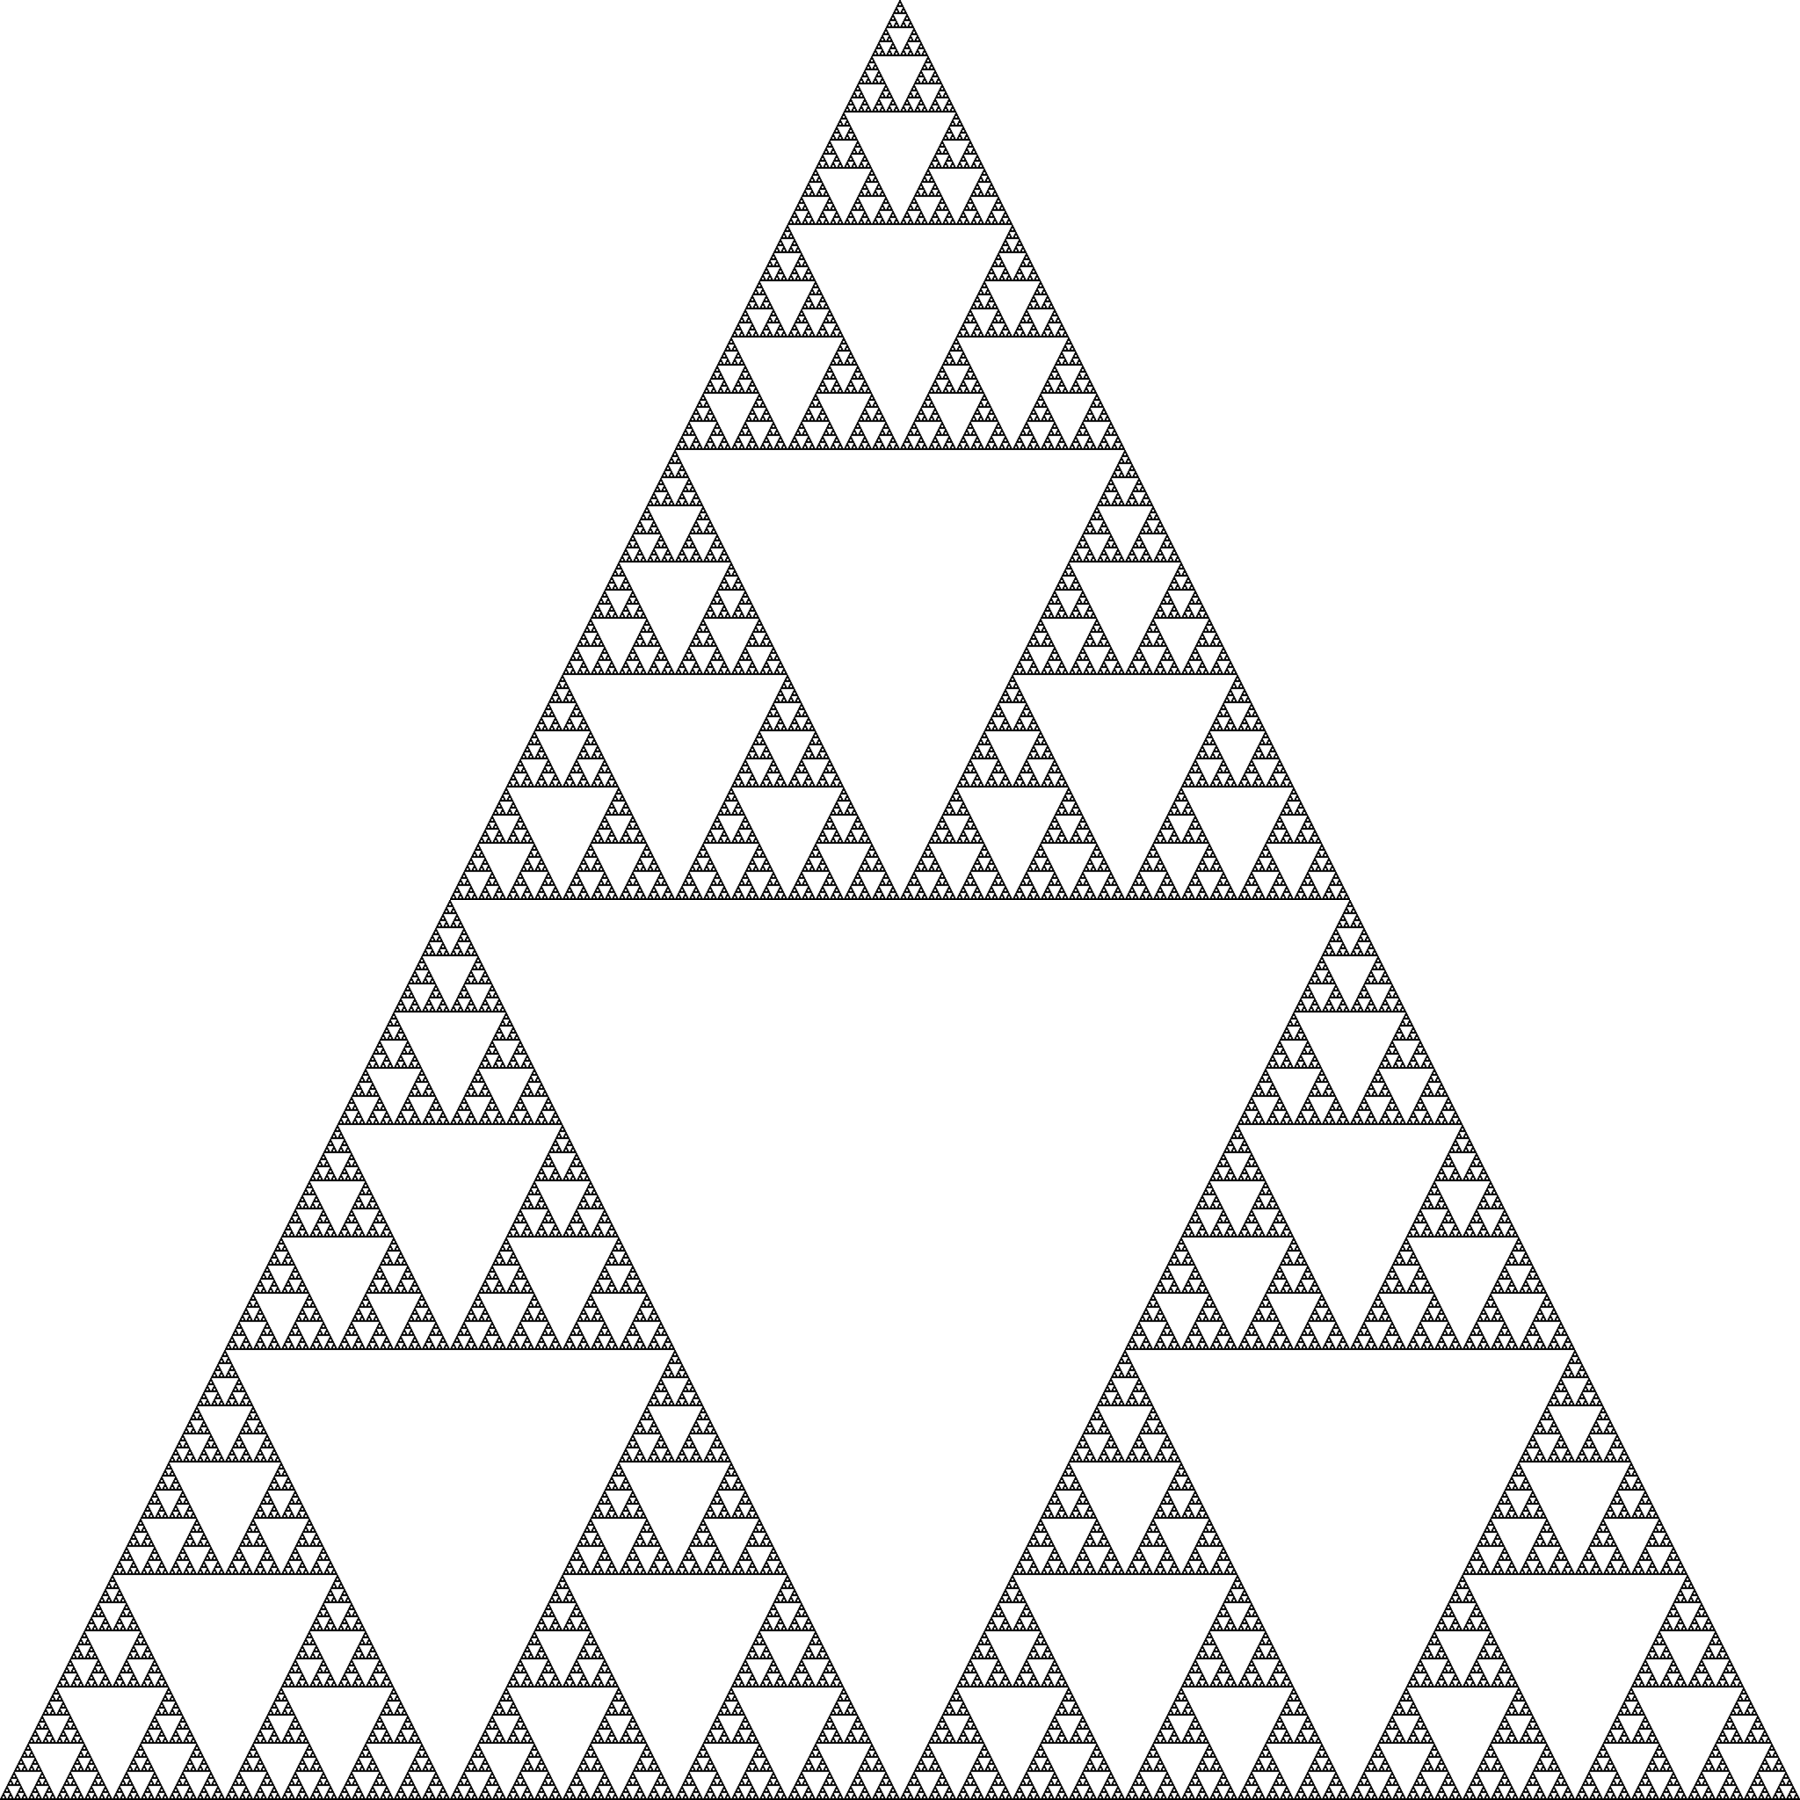
\includegraphics[width=0.5\textwidth]{papers/ifs/images/sierpinski}
	\caption{Sierpinski-Dreieck}
	\label{ifs:sierpinski10}
\end{figure}
Es besteht aus drei kleineren Kopien von sich selbst.
Es ist also ein Selbstähnliches Gebilde.
Diese Eigenschaft wollen wir uns zunutze machen.


Wir definieren das Dreieck mit Kantenlänge 1 als Menge $X$.
Ausserdem bestimmen wir drei Funktionen
\begin{align*}
	f_1(x,y)
	= 
	\begin{pmatrix}
		\frac{1}{2} & 0 \\
		0 & \frac{1}{2} \\
	\end{pmatrix}
	\begin{pmatrix}
		x\\
		y\\
	\end{pmatrix} 
	,\quad
	f_2(x,y)
	= 
	\begin{pmatrix}
		\frac{1}{2} & 0 \\
		0 & \frac{1}{2} \\
	\end{pmatrix}
	\begin{pmatrix}
		x\\
		y\\
	\end{pmatrix} 
	+
	\begin{pmatrix}
		\frac{1}{2} \\
		0
	\end{pmatrix}
	, \quad
	f_3(x,y)
	= 
	\begin{pmatrix}
		\frac{1}{2} & 0 \\
		0 & \frac{1}{2} \\
	\end{pmatrix}
	\begin{pmatrix}
		x\\
		y\\
	\end{pmatrix} 
	+
	\begin{pmatrix}
		\frac{1}{4} \\
		\frac{1}{2}
	\end{pmatrix},
\end{align*}
welche die gesamte Menge auf eine ihrer kleineren Kopien abbildet
$f_1$ bildet das Dreieck auf das Teilstück unten links ab, $f_2$ auf das Teilstück unten rechts und $f_3$ auf das obere Teilstück.
Wendet man alle drei Funktionen auf das Sierpinski-Dreieck an
\begin{align*}
	X = \bigcup\limits_{i = 1}^{3} f_i(X),
\end{align*}
entsteht also wieder ein Sierpinski-Dreieck.
Man kann sogar noch einen Schritt weiter gehen, und sagen: Wenn wir die Funktionen auf eine beliebige Startmenge anwenden, konvergiert die Menge gegen das Sierpinski-Dreieck.
\begin{figure}	
	\centering
	\subfigure[]{
		\label{ifs:sierpconsta}
		
\includegraphics[width=0.25\textwidth]{papers/ifs/images/sierpinski1}}
	\subfigure[]{
		\label{ifs:sierpconstb}
		
\includegraphics[width=0.25\textwidth]{papers/ifs/images/sierpinski2}} 
	\subfigure[]{
		\label{ifs:sierpconstc}
		
\includegraphics[width=0.25\textwidth]{papers/ifs/images/sierpinski3}}
	\subfigure[]{
		\label{ifs:sierpconstd}
		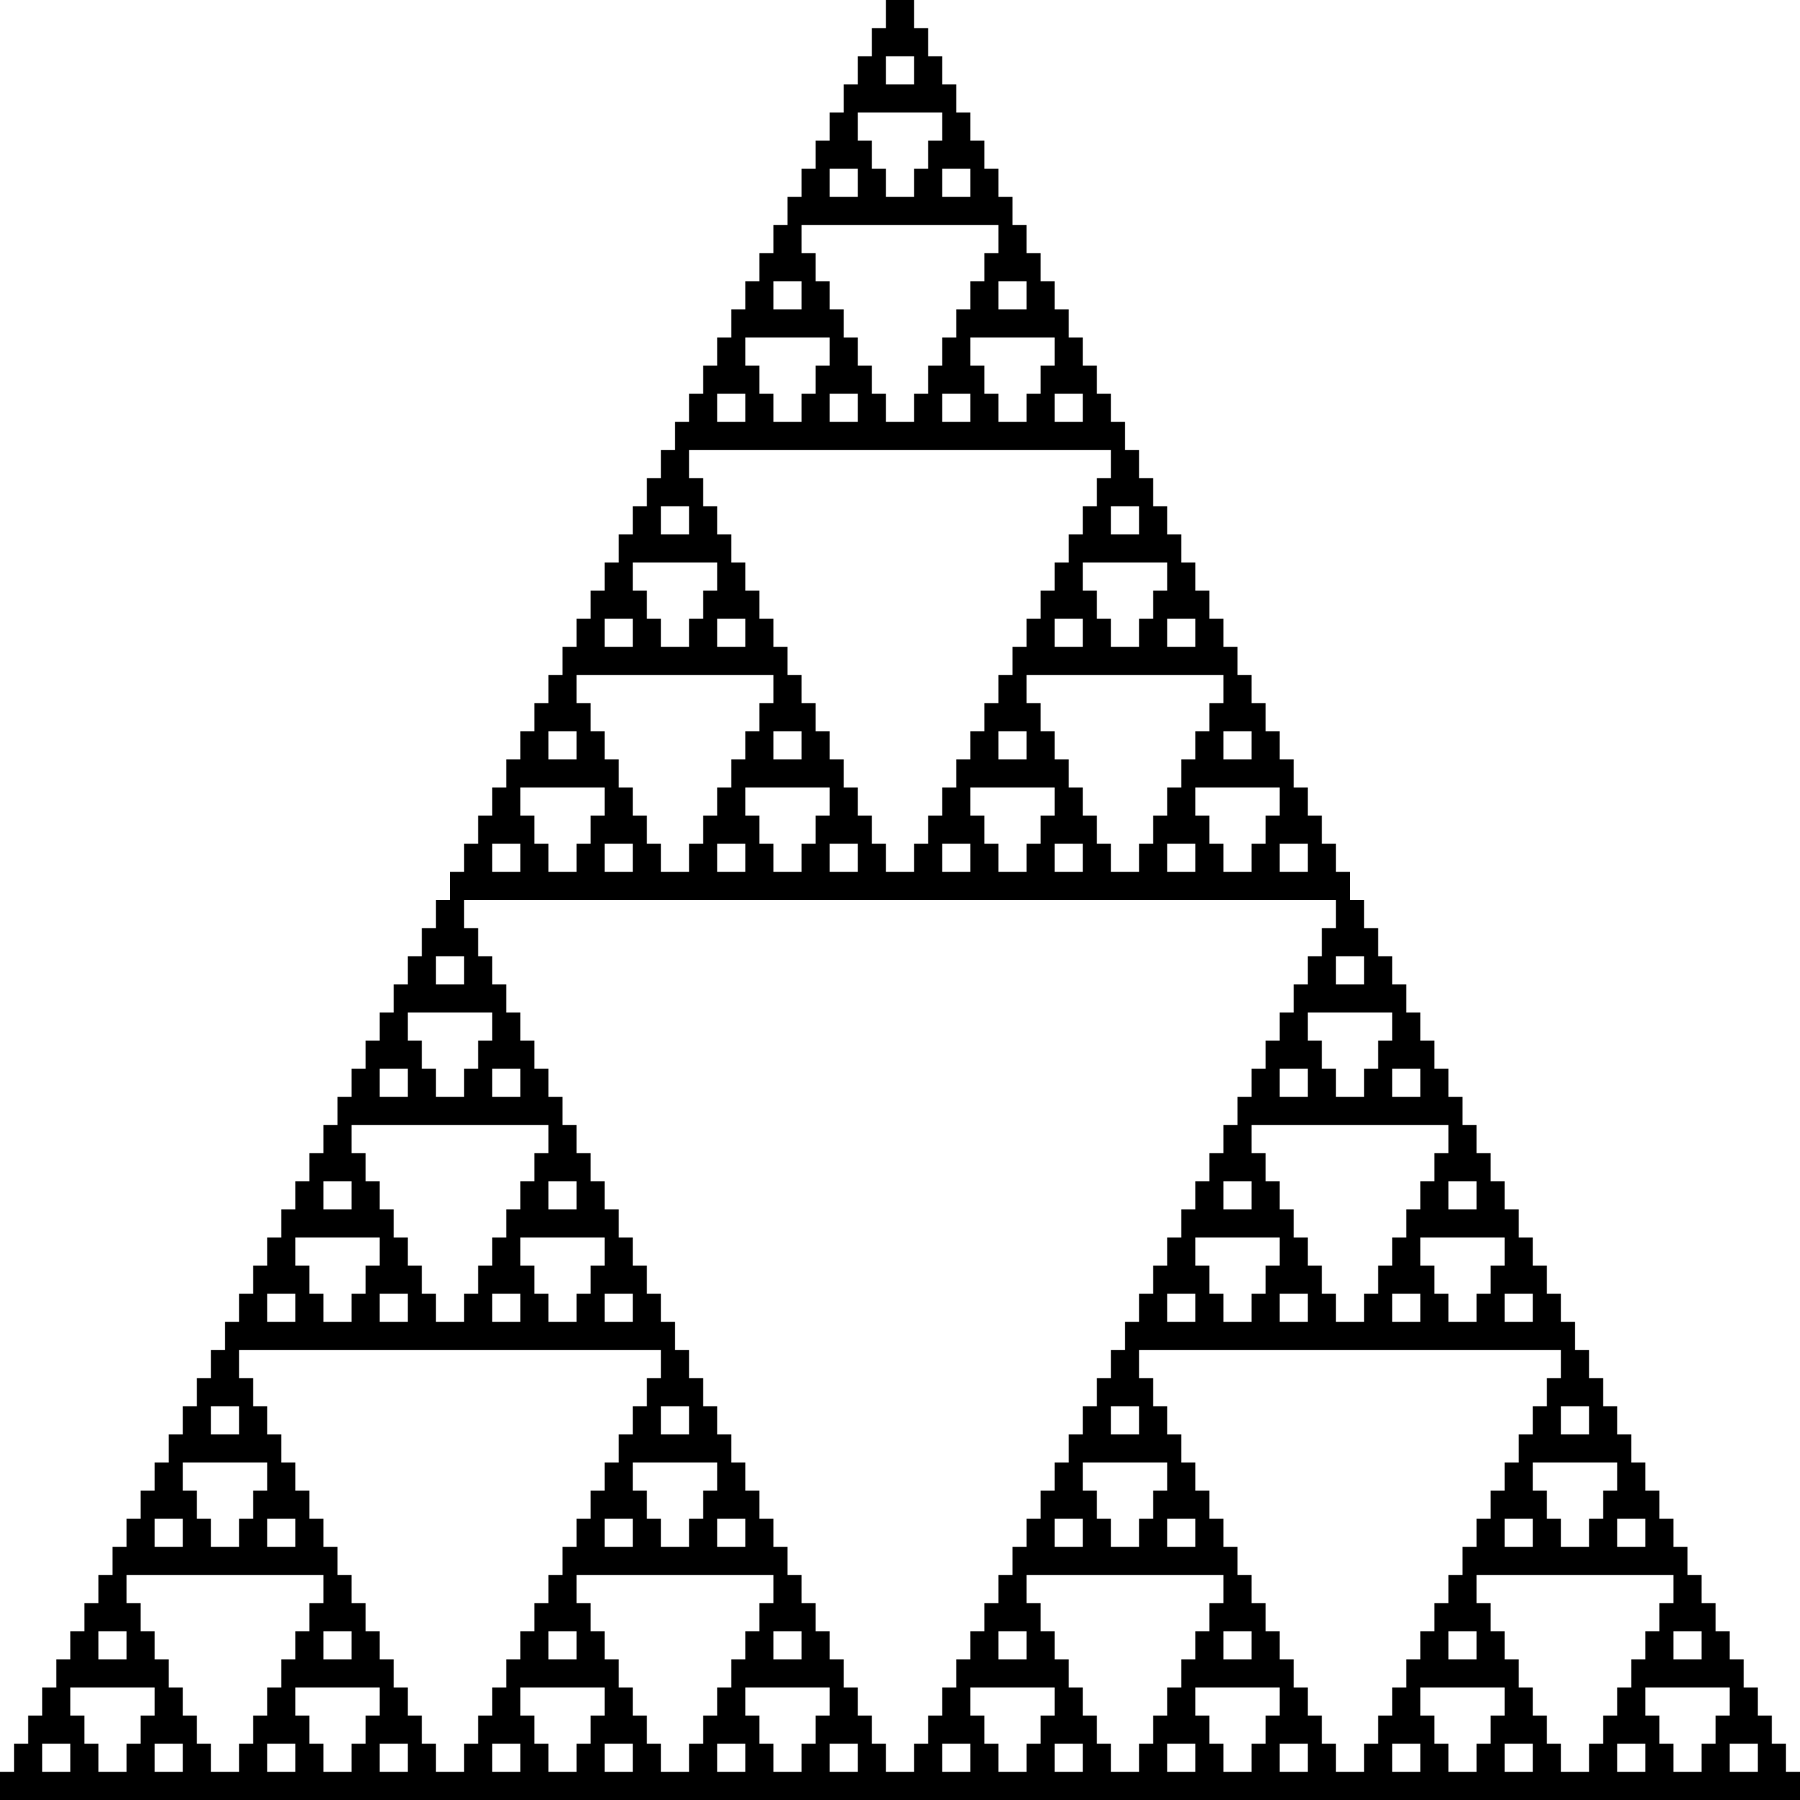
\includegraphics[width=0.25\textwidth]{papers/ifs/images/sierpinski6}}
	\caption{Konstruktion eines Sierpinski-Dreiecks mit einem Schwarzen Quadrat als Start\\
		(a) 1. Iteration (b) 2. Iteration (c) 3. Iteration (d) 5. Iteration}
	\label{ifs:sierpconst}
\end{figure}
Im Beispiel der Abbildung \ref{ifs:sierpconst} sehen wir, wie das Bild nach jeder Iteration dem Sierpinski-Dreieck ähnlicher wird.
Der Abstand zum Original wird immer kleiner, und konvergiert gegen null.

\subsection{Iterierte Funktionensysteme
\label{ifs:subsection:bonorum}}
In diesem Abschnitt wollen wir die Erkenntnis, wie wir aus einer beliebigen Menge ein Sierpinski-Dreieck generieren können, verallgemeinern.


$S_1,...,S_n$ sind Kontraktionen auf die Menge $D \subset \mathbb{R}^n$. Es gilt
\begin{align}
	|S_i(x) - S_i(y)| \leq c_i|x - y|
\end{align}
für jedes i mit einem $c_i < 1$. Dann existiert eine eindeutige kompakte Menge $F$ für die gilt
\begin{equation}
	F = \bigcup\limits_{i = 1}^{m} S_i(F)
\end{equation}
Weiter definieren wir die Transformation S auf kompakte Mengen ohne die leere Menge.
\begin{equation}
	S(E) = \bigcup\limits_{i = 1}^m S_i(E)
\end{equation}
Wird diese Transformation Iterativ ausgeführt, das heisst $S^0(E) = E, S^k(E) = S(S^{k-1}(E))$, und für jedes $i$ $S_i(E) \subset E$, gilt
\begin{equation}
	F = \bigcap\limits_{k = 1}^{\infty} S^k(E).
\end{equation}
In Worte gefasst bedeutet das, dass jede Gruppe von Kontraktionen iterativ ausgeführt, gegen eine eindeutige Menge konvergiert.
Diese Menge ist auch als Attraktor des IFS bekannt.
Dies für jede Startmenge, solange diese ihre Transformierten wieder beinhaltet.
Auf den Beweis wird verzichtet.
\subsection{Beispiel: Barnsley-Farn}
Der Barnsley-Farn, Abbildung \ref{ifs:farn}, ist ein Beispiel eines Fraktal, welches mit einem IFS generiert werden kann.
Wie man schnell erkennen kann, besteht der Farn aus Blättern, welche eine grosse Ähnlichkeit zum ganzen Farn haben.
\begin{align*}
	{S_1(x,y)}
	= 
	\begin{pmatrix}
		0 & 0 \\
		0 & 0.16 \\
	\end{pmatrix}
	\begin{pmatrix}
		x\\
		y\\
	\end{pmatrix}, \quad
	{S_2(x,y)}
	= 
	\begin{pmatrix}
		0.85 & 0.04 \\
		-0.04 & 0.85 \\
	\end{pmatrix}
	\begin{pmatrix}
		x\\
		y\\
	\end{pmatrix} 
	+
	\begin{pmatrix}
		0 \\
		1.6
	\end{pmatrix}\\
	{S_3(x,y)}
	= 
	\begin{pmatrix}
		0.2 & -0.26 \\
		0.23 & 0.22 \\
	\end{pmatrix}
	\begin{pmatrix}
		x\\
		y\\
	\end{pmatrix} 
	+
	\begin{pmatrix}
		0 \\
		1.6
	\end{pmatrix}, \quad
	{S_4(x,y)}
	= 
	\begin{pmatrix}
		-0.15 & 0.28 \\
		0.26 & 0.24 \\
	\end{pmatrix}
	\begin{pmatrix}
		x\\
		y\\
	\end{pmatrix} 
	+
	\begin{pmatrix}
		0 \\
		0.44
	\end{pmatrix}\\
\end{align*}
In der Abbildung \ref{ifs:farncolor} sehen wir die vier Transformationen farblich dargestellt.

$S_1$ erstellt den Stiel des Farnblattes (rot).
Die Transformation bildet das Gesamte Blatt auf die Y-Achse ab.
$S_2$ (grün) erstellt den Hauptteil des Farnes. 
Sie verkleinert und dreht das gesamte Bild und stellt es auf das Ende des Stiels aus $S_1$.
$S_3$ bildet das gesamte Blatt auf das blaue Teilblatt unten Links ab.
$S_4$ spiegelt das Blatt und bildet es auf das magentafarbene Teilblatt ab.  
\subsection{Chaosspiel}
Wir führen im Zusammenhang mit dem Barnsley-Farn \cite{ifs:barnsleyfern} noch eine weitere Methode ein, um ein IFS zu zeichnen.
Bis jetzt wurde immer davon gesprochen, die Transformationen auf die gesamte Menge anzuwenden.
Bei komplizierteren IFS welche viele Iterationen brauchen, bis man den Attraktor erkennen kann, ist diese Methode ziemlich rechenintensiv.
Eine Alternative ist das Chaosspiel \cite{ifs:chaos}. 
Bei dieser Methode werden die Transformationen nicht auf die Menge angewendet, sondern nur auf einen einzelnen Punkt.
Der Startpunkt kann dabei ein beliebiger Punkt in $E$ sein.
Es wird bei jedem Iterationsschritt nur eine Transformation, welche zufällig gewählt wurde, angewendet.
Da, wie wir beim Barnsley-Farn gut sehen, dass nicht jede Transformation gleich viel des Bildes ausmacht, werden diese beim Chaosspiel gewichtet.
Die Gewichtung erfolgt über den Anteil der Gesamtmasse.
Im Fall des Barnsley-Fern wird $S_1$ in $1\%$, $S_2$ in $85\%$ und $S_3 \& S_4$ in $7\%$ der Iterationen ausgeführt. 
\begin{figure}	
	\centering
	\makebox[\textwidth][c]{
		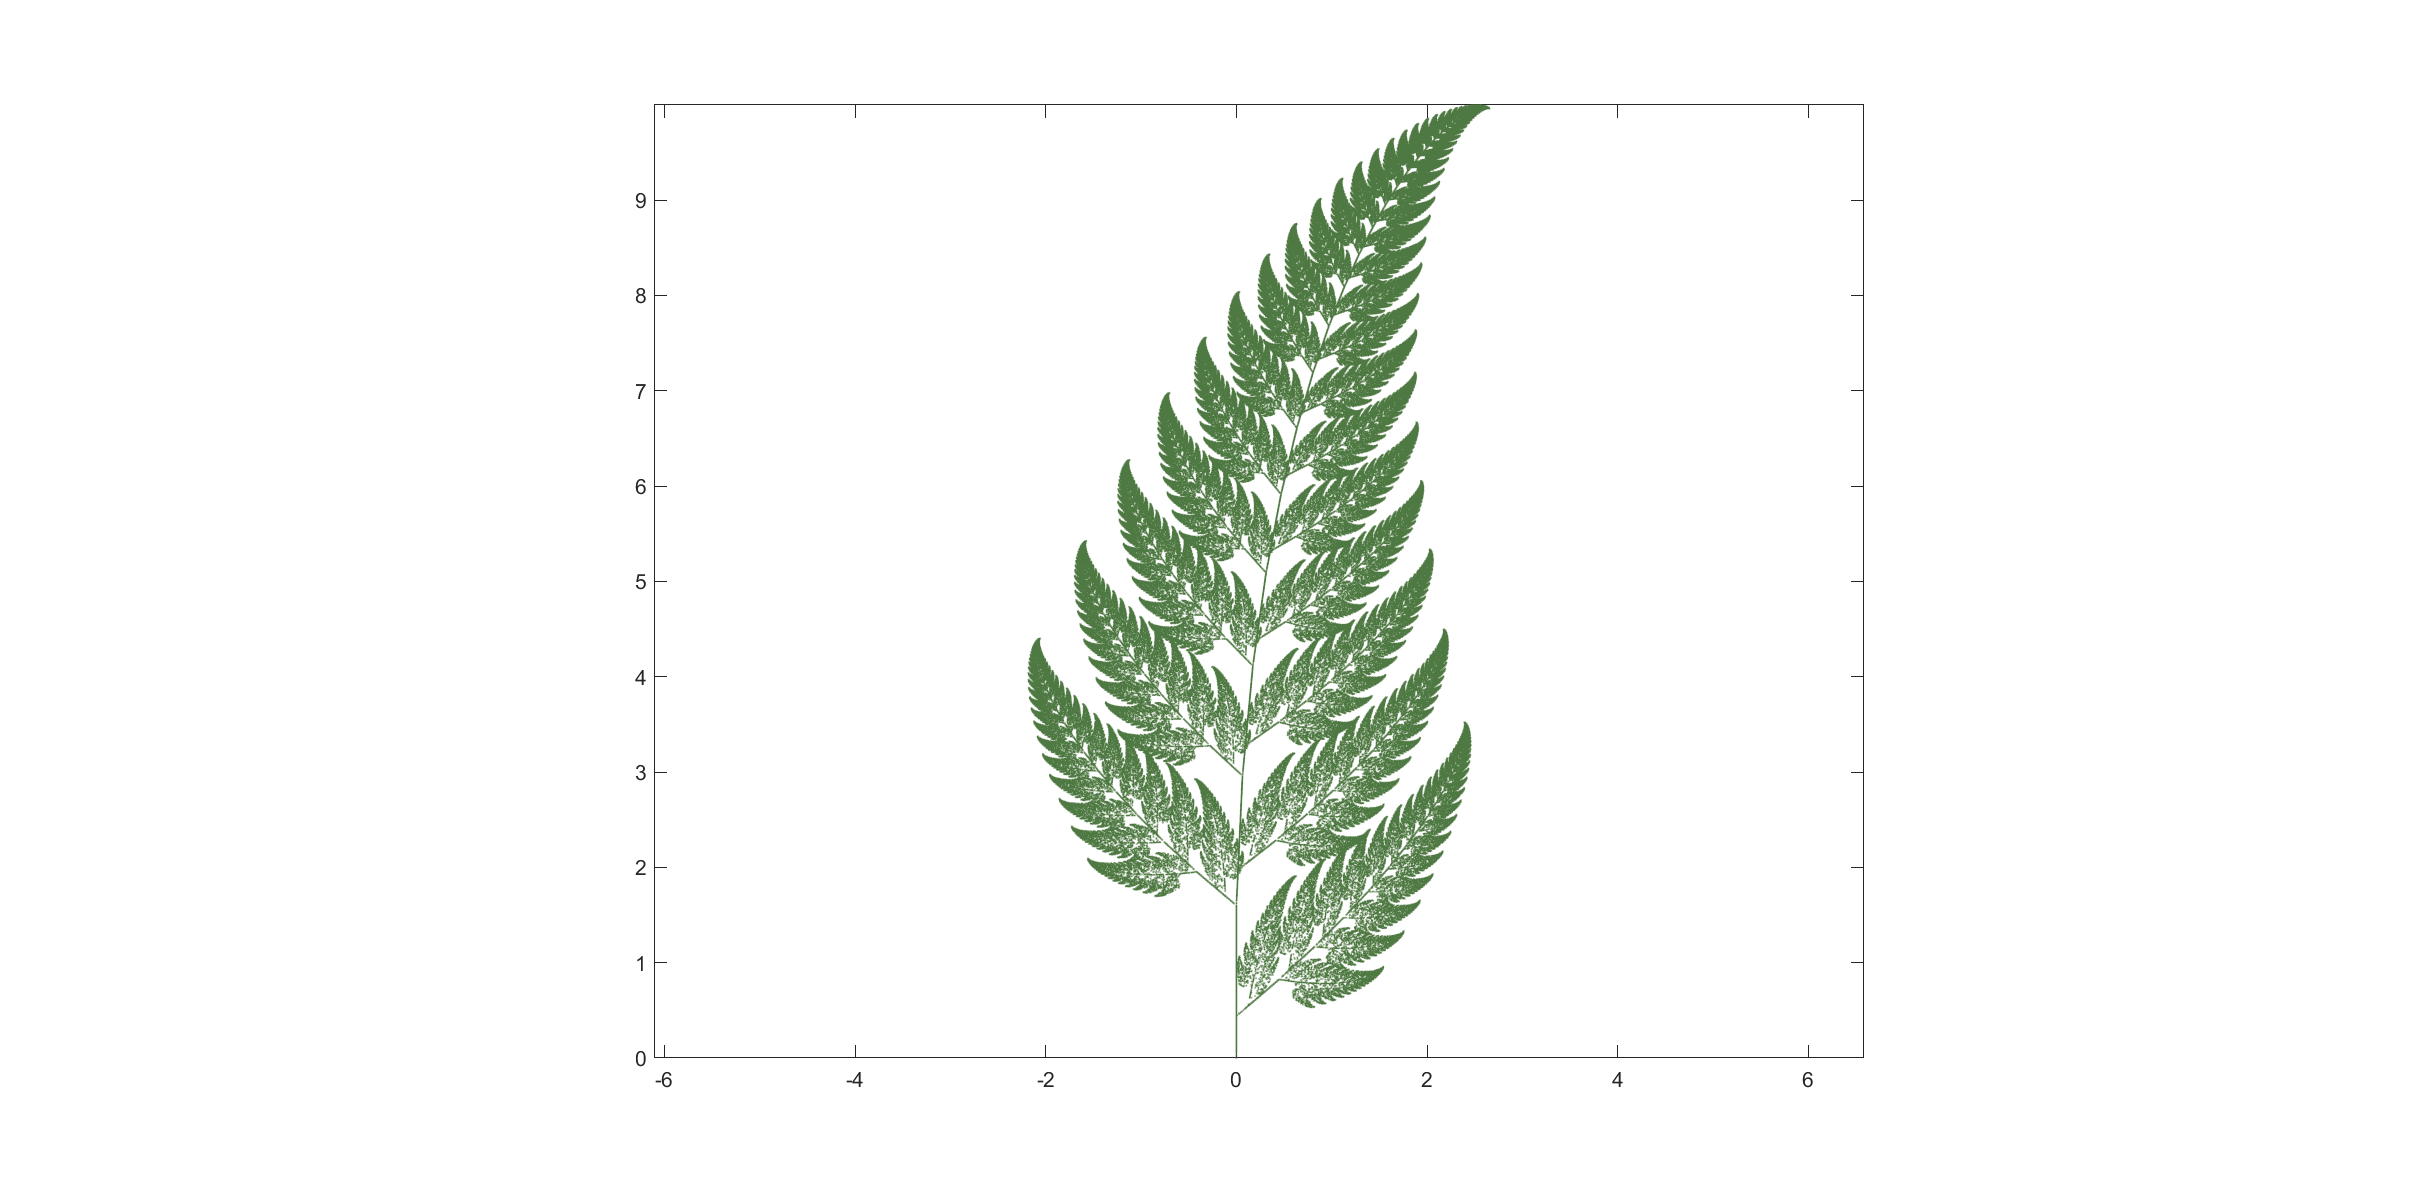
\includegraphics[width=1.4\textwidth]{papers/ifs/images/farn}}
	\caption{Barnsley-Farn}
	\label{ifs:farn}
\end{figure}
\begin{figure}
	\centering
	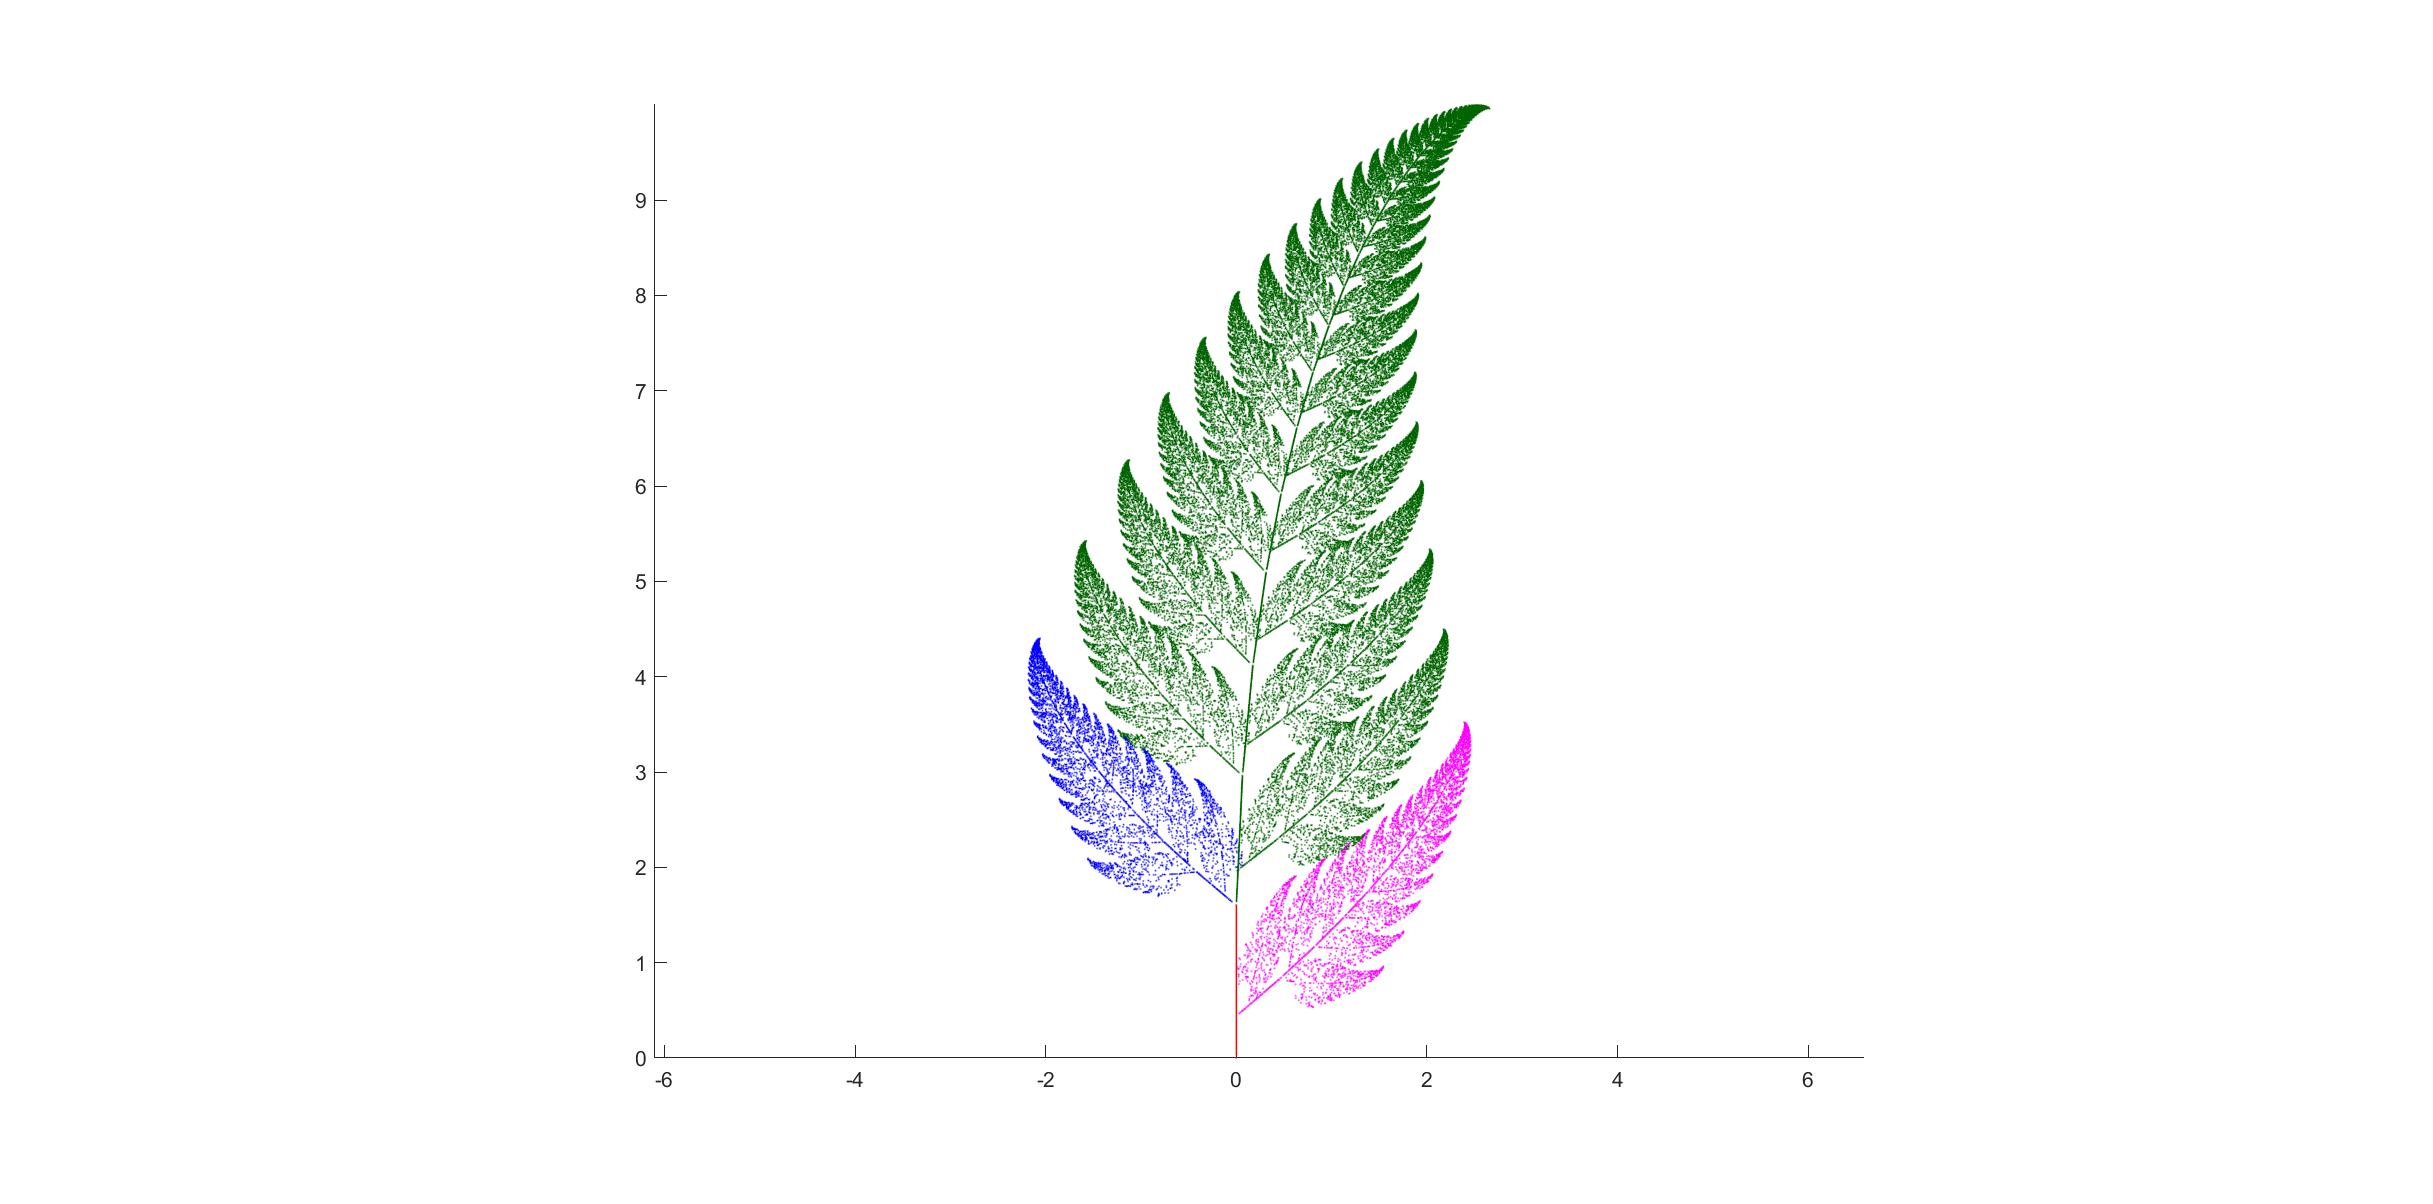
\includegraphics[width=0.7\textwidth]{papers/ifs/images/farncolor}
	\caption{Vier Transformationen des Barnsley-Farn}
	\label{ifs:farncolor}
\end{figure}
\begin{figure}	
	\centering
	\makebox[\textwidth][c]{
		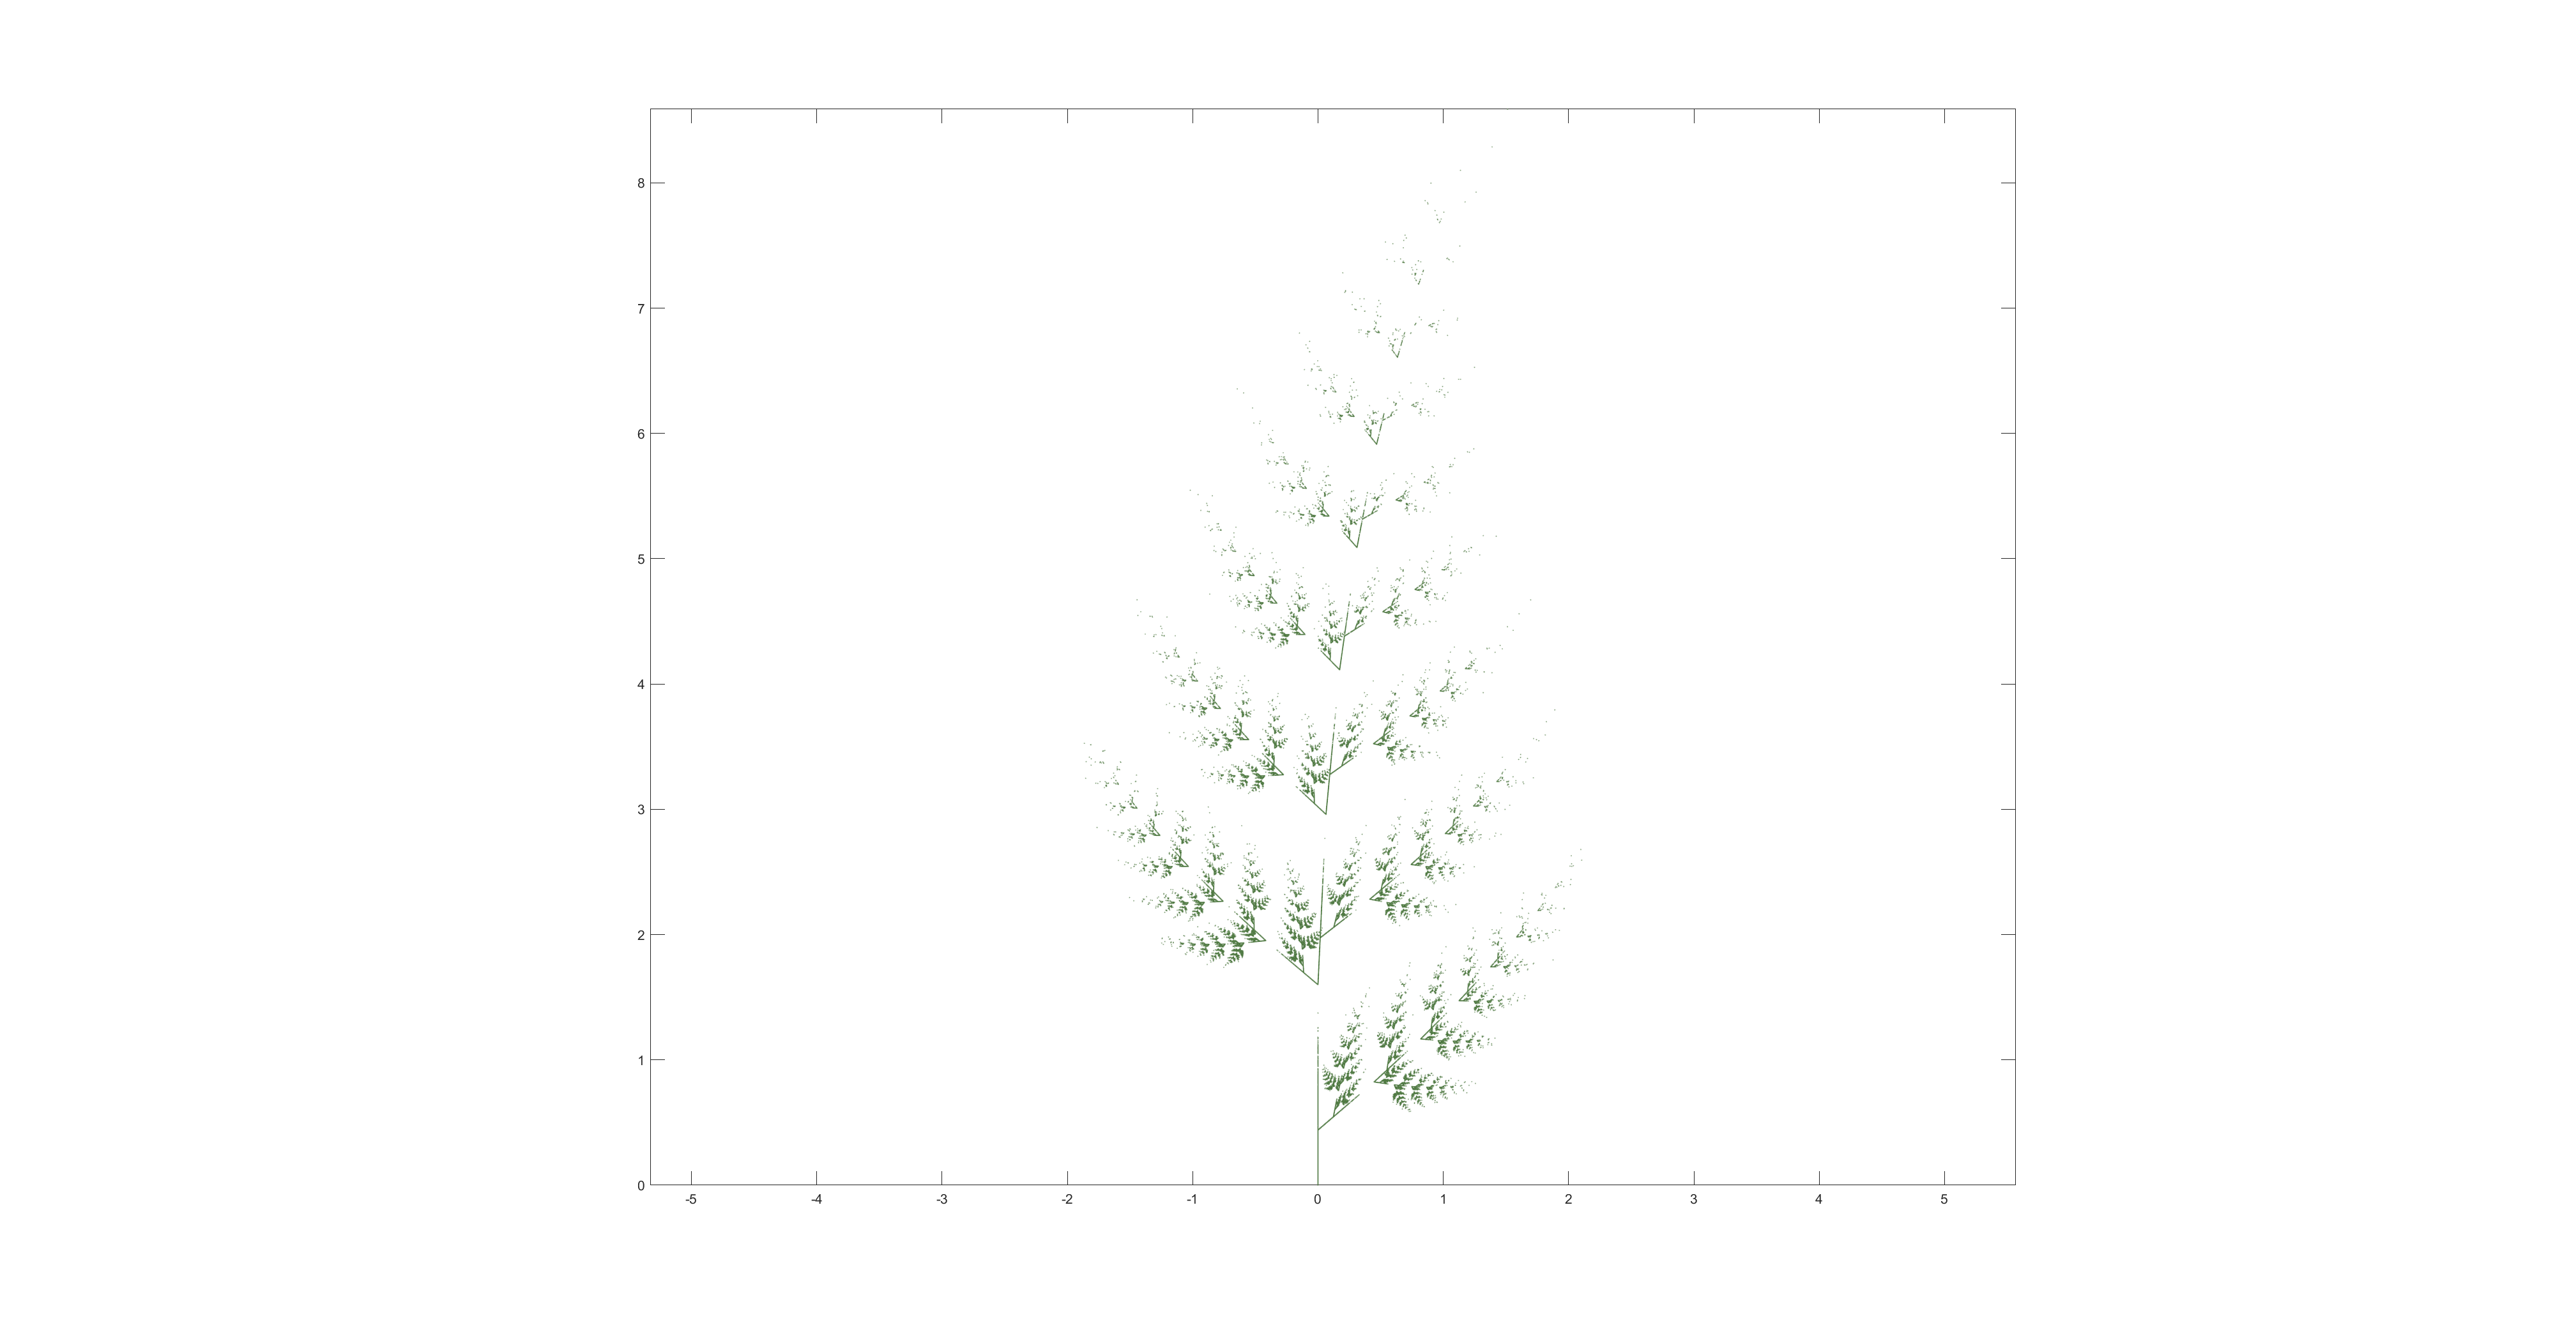
\includegraphics[width=1.4\textwidth]{papers/ifs/images/farnnotweight}}
	\caption{Chaosspiel ohne Gewichtung}
	\label{ifs:farnNoWeight}
\end{figure}

%
% teil3.tex -- Beispiel-File für Teil 3
%
% (c) 2020 Prof Dr Andreas Müller, Hochschule Rapperswil
%
\section{Der Munkres-Algorithmus oder die ungarische Methode
\label{munkres:section:teil3}}

Mit der ungarischen Methode können also Optimierungsprobleme gelöst
werden, die bei gewichteten Zuordnungen in bipartiten Graphen entstehen.
Mit ihr kann die eindeutige Zuordnung von Objekten aus zwei Gruppen so
optimiert werden, dass die Gesamtkosten minimiert werden bzw.~der
Gesamtgewinn maximiert werden kann.

\rhead{Ungarische Methode}

\subsection{Geschichte
\label{munkres:subsection:malorum}}
Die Ungarische Methode wurde 1955 von Harold Kuhn entwickelt und veröffentlicht.
\index{Kuhn, Harold}%
Der Name ``Ungarische Methode'' ergab sich, weil der Algorithmus
weitestgehend auf den früheren Arbeiten zweier ungarischer Mathematiker
basierte: Dénes Kőnig und Jenő Egerváry.
\index{Konig, Denes@Kőnig, Dénes}%
\index{Egerváry, Jenő}%
\index{Munkres, James}%
James Munkres überprüfte den Algorithmus im Jahr 1957 und stellte fest,
dass der Algorithmus (stark) polynomiell ist.
Seitdem ist der Algorithmus auch als Kuhn-Munkres- oder
Munkres-Zuordnungsalgorithmus bekannt.
\index{Kuhn-Munkres-Zuordnungsalgorithmus}%
\index{Munkres-Zuordnungsalgorithmus}%
Die Zeitkomplexität des ursprünglichen Algorithmus war $O(n^4)$,
später wurde zudem festgestellt, dass er modifiziert werden kann,
um eine  $O(n^3)$-Laufzeit zu erreichen.

\subsection{Besondere Leistung der Ungarischen Methode
\label{munkres:subsection:malorum}}
Die ungarische Methode ist ein kombinatorischer Optimierungsalgorithmus, der das Zuordnungsproblem
\index{Optimierungsalgorithmus, kombinatorisch}%
in polynomieller Zeit löst.
Der Begriff polynomielle Laufzeit bedeutet, dass die Laufzeit des Programms
\index{polynomielle Laufzeit}%
wie $n^2$, $n^3$, $n^4$, etc.~wächst und vernünftig skaliert. $n$ ist hierbei die ``Grösse'' des Problems.

\subsection{Unterschiedliche Anzahl von Quellen und Zielen
\label{munkres:subsection:malorum}}
Es gibt Fälle, in welchen das Ausgangsproblem keine quadratische Form besitzt.
Das ist z.~B.~dann der Fall, wenn drei Mitarbeiter vier verschiedene Eignungstests absolvieren müssen.
In diesem Fall wird in der Ungarischen Methode die Matrix künstlich mittels einer Dummy-Position zu einem Quadrat ergänzt.
Dummy-Positionen werden dann mit der größten vorhandenen Zahl aus der Matrix besetzt.
Beispielsweise wird eine $3\times 4$ zu einer $4\times 4$-Matrix.

\subsection{Beispiel eines händischen Verfahrens
\label{munkres:subsection:malorum}}
\begin{figure}
\centering
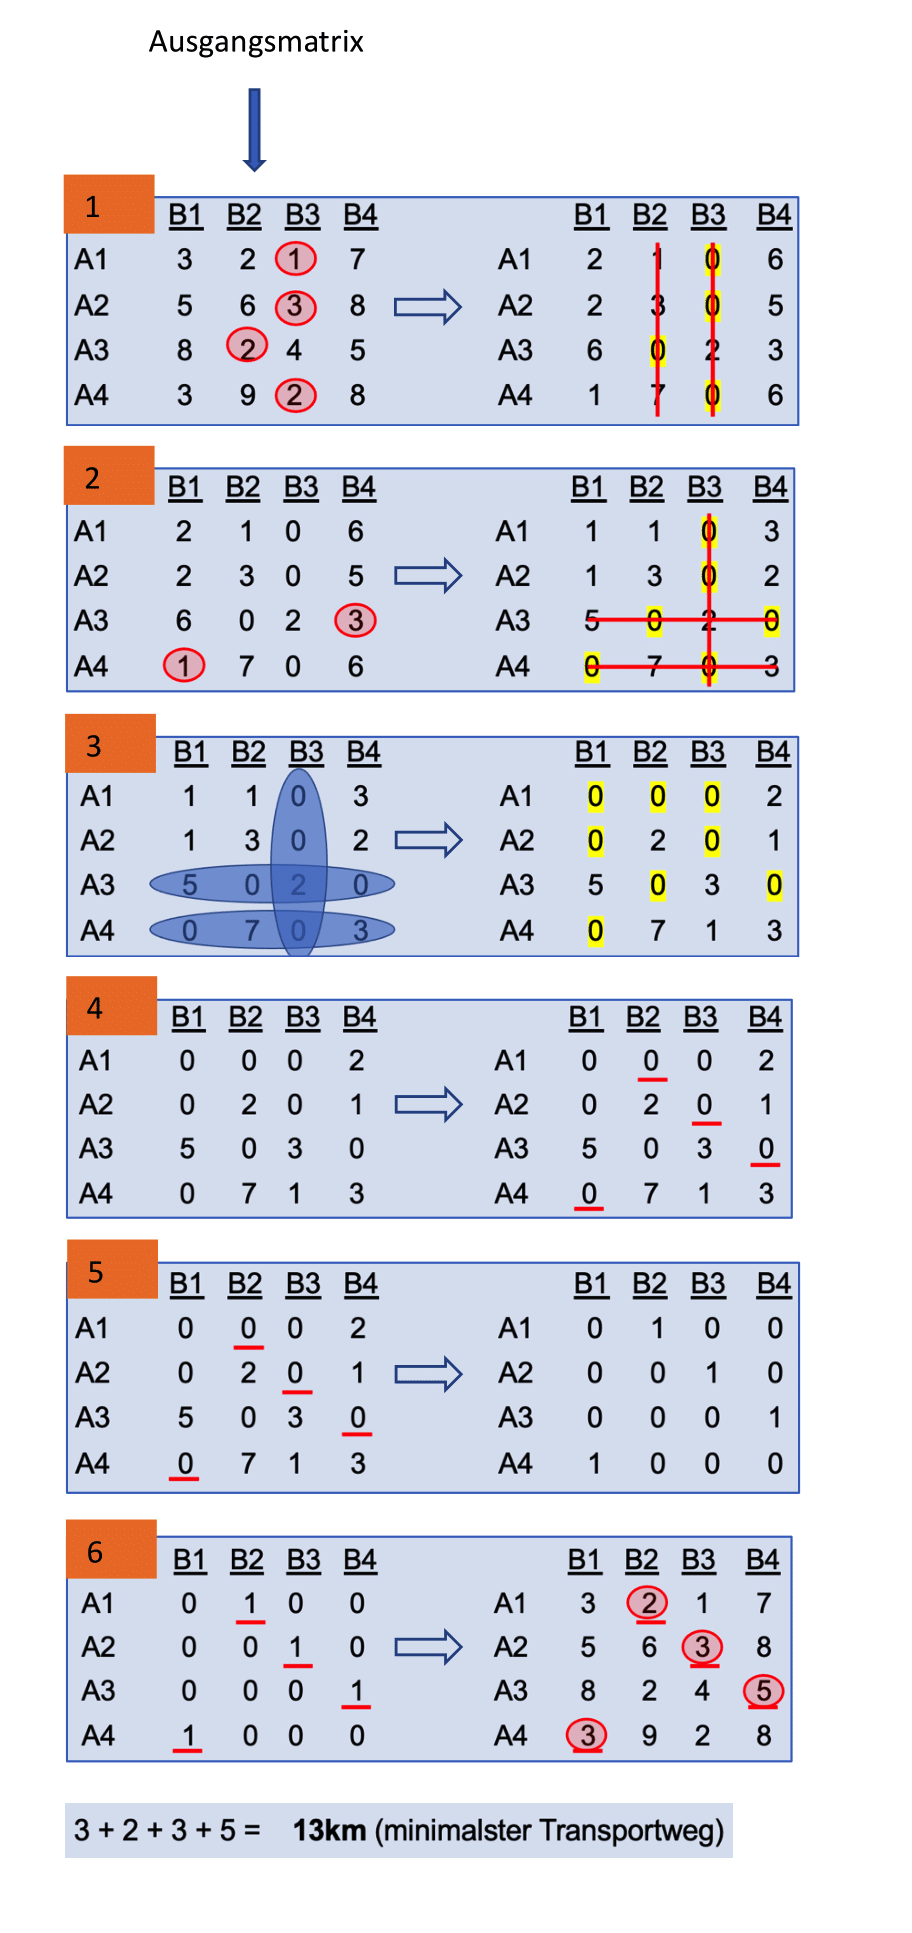
\includegraphics[width=8cm]{papers/munkres/figures/Ungarische_Methode_Beispiel.png}
\caption{Händisches Beispiel des Munkres Algorithmus, minimaler Transportweg.}
\label{munkres:Vr2}
\end{figure}

Die ungarische Methode kann in einem einfachen händischen Beispiel erläutert werden. Wir gehen von der Kostenmatrix $A$ aus. Diese Matrix wird in mehreren Schritten immer weiter reduziert. Anschliessend erfolgen mehrere Zuordnungen. Hierbei ist zu beachten, dass jede Zeile und jede Spalte immer genau eine eindeutige Zuordnung ergibt. Es gibt Situationen, in denen man nichts mehr tun muss, um eine optimale Zuordnung zu finden. Eine optimale Zuordnung ohne zusätzliche Kosten ist eine Auswahl genau eines Feldes in jeder Zeile und Spalte, welches 0 enthält. Das Ziel des Algorithmus ist also, die Matrix so zu ändern, dass genügend Nullen in der Matrix vorkommen. Es ist zudem wichtig, dass man nach jeder Modifikation der Matrix testet, ob man bereits eine Zuordnung machen kann, also genügend Nullen hat.
Das Vorgehen wird in den nachfolgenden Schritten 1--6 beschrieben und auch in der Abbildung 21.5 dargestellt.

\begin{enumerate}
\item Man beginnt mit der Zeilen-Reduktion. Pro Zeile eruiert man die kleinste Zahl. Diese kleinste Zahl, jeweils in rot markiert, wird bei allen anderen Ziffern in der jeweiligen Zeile subtrahiert. Mit dieser Subtraktion zieht man die unvermeidbaren Kosten ab, die man hat, um eine Baustelle zu erreichen. Man erkennt, dass die Nullen mit zwei Linien abdeckbar sind. Das heisst es gibt zwei Spalten bei denen noch keine Zuordnungen möglich sind. 

\item Auch im zweiten Schritt werden mittels der Spalten-Reduktion die unvermeidbaren Weg-Kosten abgezogen. Man zieht die kleinste Zahl, wiederum in rot markiert, in jeder Spalte von allen Zahlen in der Spalte ab.
Die Nullen können somit mit drei Linien abgedeckt werden. Im Idealfall hat die Matrix in jeder Zeile und Spalte bereits genügend viele Nullen, so dass man bereits eine Zuordnung ohne Mehrkosten machen kann. Dies ist jedoch noch nicht der Fall. Es sollen weitere Nullen in die Matrix hineingebracht werden.

\item Es bleiben jetzt einige Felder übrig, für die noch keine Zuordnung möglich ist. Die kleinste Ziffer wird dabei aus den noch nicht mit blau markierten Zahlen ausgewählt werden. Im Beispiel ist es die Zahl 1. Das Feld mit dem kleinsten Eintrag beinhaltet die Kosten, die unvermeidlich sind, wenn man für diese Felder auch noch eine Zuordnung machen will. Um neue Nullen zu bekommen, lagert man jetzt die Kosten auf die anderen Zeilen und Spalten um. Dies tut man, indem man in allen nicht abgedeckten Feldern die minimalen Kosten subtrahiert und in den blau markierten Kreuzungspunkten dazu addiert.
Dieser Schritt 3 muss so oft wiederholt werden, bis genügend viele Nullen in der Matrix vorhanden sind.

\item In Schritt 4 sollen jetzt möglichst viele Nullen markiert werden, welche freistehend sind.
Freistehend bedeutet, dass sowohl in der jeweiligen Zeile und Spalte keine andere markierte Null vorhanden ist.

\item Alle markierten Nullen werden jetzt in eine 1 umgewandelt. Die restlichen Ziffern in der Matrix, exklusiv die Einsen, sollen jetzt ignoriert und durch eine 0 ersetzt werden.

\item Zu guter Letzt werden überall wo eine 1 steht, die Zahlen aus der Ausgangsmatrix eingefügt. Nach Einsetzen der Zahlen können die in rot markierten Zahlen aufsummiert werden. Man erhält den minimalen Transportweg von total 13 Kilometer.
\end{enumerate}

\begin{figure}
\centering
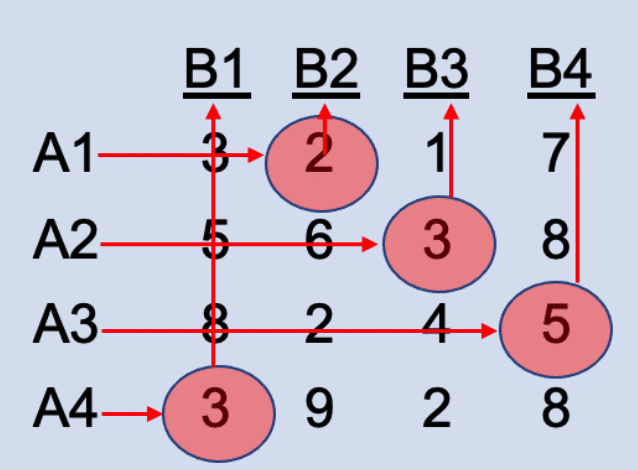
\includegraphics[width=3cm]{papers/munkres/figures/Ungarische_Methode_Beispiel_Zuw.png}
\caption{Händisches Beispiel des Munkres Algorithmus, Zuweisung der Kräne }
\label{munkres:Vr2}
\end{figure} 

\subsection{Zuordnung der Kräne
\label{munkres:subsection:malorum}}

Als Resultat des Munkres-Algorithmus werden in Abbildung 21.6 nebst dem minimalen Transportweg auch die optimale Zuweisung der Kräne auf die neuen Standorte ersichtlich.
Es können die folgenden Zuordnungen aus der Matrix abgelesen werden:
\begin{itemize}
\item Der Kran von Baustelle A1 soll zur Baustelle B2.
\item Der Kran von Baustelle A2 soll zur Baustelle B3.
\item Der Kran von Baustelle A3 soll zur Baustelle B4.
\item Der Kran von Baustelle A4 soll zur Baustelle B1.
\end{itemize}



\printbibliography[heading=subbibliography]
\end{refsection}
